\section{Problem (5)}
	The body in \cref{fig:hwa_problem5} is pivoted at $O$. Three forces act on it in the directions shown: $F_{A} = \ 9.3 \ N$ at point $A$, $7.5 \ m$ from $O$; $F_{B} = \ 11.0 \ N$ at point $B$, $5.4 \ m$ from $O$; and $F_{C} = \ 8.8 \ N$ at point $C$, $4.4 \ m$ from $O$. Taking the clockwise direction to be negative, what is the net torque about $O$?

	\begin{figure}[H]
		\begin{center}
			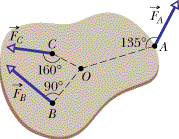
\includegraphics[scale=1]{hwa_problem5}
			\caption{Illustration of Problem 5}
			\label{fig:hwa_problem5}
		\end{center}
	\end{figure}

	\textbf{R:}

	\begin{align}
		x
	\end{align}
